% ============================================================
% 片段：s02a  对应原文 section2.tex 第 1--354 行；PDF 第 6--15 页
% 内容：§2 Higher-Form Symmetry（2.1--2.2）
% 译者：t-s02a   审校状态：初稿
% ============================================================

% ==== 原文 PDF 第 6 页 ====
\section{高形式对称性}\label{sec:higher-form-gen}

\begin{keytakeaways}
  \begin{itemize}[leftmargin=1.4em,itemsep=2pt,topsep=2pt]
    \item \textbf{物理图像}：在 QFT 中，对称性的生成元应被理解为拓扑算符 $U_g(X)$：其相关函数在支撑流形 $X$ 的连续形变下不变。量子力学中 $U_g$ 沿时间轴移动不受阻碍，这一“拓扑性”在更高维中表现为对任意形变的不变性。
    \item \textbf{数学工具}：把支撑流形的余维从 $1$ 提高到 $p+1$、并把局域算符换成 $p$ 维延展对象，即得 $p$-形式对称性；其作用律以环绕数 $\langle M^{d-p-1},C^{p}\rangle=1$ 为条件，而环绕数可等价地用交点数 $\mathrm{Int}(X^{d-p},C^{p})=\mathrm{Int}(M^{d-p-1},Y^{p+1})$ 计算。
    \item \textbf{关键结论}：$p>0$（且时空拓扑平凡）时高形式对称性必然阿贝尔——余维 $\ge2$ 的拓扑算符可在时空中作拓扑互换；$p=0$ 时两个算符支撑在不同时间切片上而无法互换，故允许非阿贝尔。
    \item \textbf{关键结论}：纯 $U(1)$ 麦克斯韦理论具有 $U(1)_E\times U(1)_M$ 1-形式对称性，$\star F$ 与 $F$ 的闭性（$\dd\star F=0$、$\dd F=0$）保证相应的拓扑算符，它们分别作用在威尔逊圈与 't Hooft 圈上并给出相位 $\mathrm{e}^{in\alpha\langle S,\gamma\rangle}$。
    \item \textbf{关键结论}：带荷物质把 $U(1)_E$ 破缺为 $\mathbb{Z}_N$（$N$ 为电荷的最大公约数），$U(1)_M$ 不受影响；非阿贝尔规范理论中，$SU(N)$ 有 $\mathbb{Z}_N$ 电中心对称性、$PSU(N)$ 有 $\mathbb{Z}_N$ 磁对称性，而互局域算符集合（极化）的选取决定理论的整体形式：绝对理论有配分函数，相对理论只有配分向量。
  \end{itemize}
\end{keytakeaways}

本节对高形式对称性（higher-form symmetry）作一基础性介绍。首先回顾与普通对称性相联系的拓扑算符（topological operator），为进一步的探讨作铺垫；随后给出高形式对称性的定义与示例。本节后半部分包括高形式对称性的规范化（gauging），以及理解高形式对称性的另外三种有用视角。

鉴于本节为后续讨论奠定基础，建议读者完整阅读这部分内容。本节力求浅显易读，目的是帮助读者在进入后面更复杂的专题之前建立起基础知识；那些专题可按各人兴趣选读。

\subsection{普通对称性中的拓扑算符}\label{sec:ordinary}

用现代的语言，对称性的生成元被描述为拓扑算符，下面就来引入这一概念。以下把时空流形记为 $M$（若要强调其 $d$ 维，则记为 $M^d$）。对称性算符记为 $U_g(X)$，其中 $g\in G$ 是对称群的群元，$X\subseteq M$ 是承载该拓扑算符的流形（后文会作解释）。

先看量子力学中的一个基本例子。

\begin{example}
    $M^{0+1} = \mb{R}$，$U_g=U_g(t)$ 是在点 $t\in \bbR$ 处定义的对称性算符。由于
    \[ [U_g,H] = 0 \ , \]
    通常选择略去其时间依赖。现考虑一个在此对称性下带荷的对象（此处即局域算符）$O_{\{ i\}}$，以及作用在该对象上的伴随作用
    \[ U_g O_i(t) U_g^{-1} = \mathcal{R}_i^j(g) O_j(t)  \]
    给出一个表示 $\mathcal{R}$。该公式的图示理解见图~\ref{Fig:0FormQM}。
\end{example}

% ==== 原文 PDF 第 7 页 ====
\begin{figure}[htbp]
  \centering
  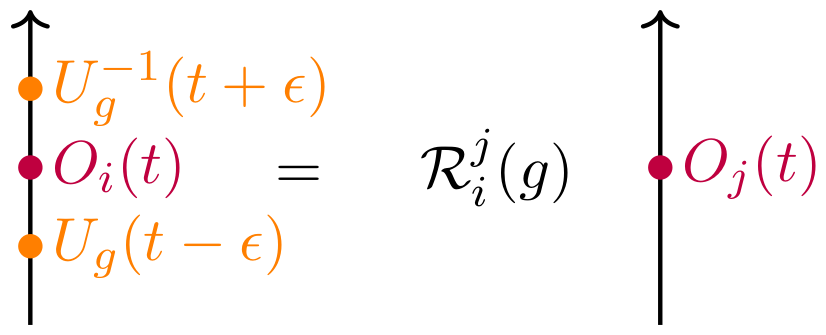
\includegraphics[width=0.32\linewidth]{figures/figure-1.png}
  % [原文图注为空]
  \caption{}
  \label{Fig:0FormQM}
\end{figure}

那么“拓扑的”究竟指什么？既然 $U_g$ 与哈密顿量对易，它就可以沿时间轴移动，只要“障碍”$\{ O_i(t)\}$ 不挡路。这一拓扑性质在更高维的例子中会表现得更为明显。

\begin{example}[$M^d$ 中的 0-形式对称性]
    为推广上例，把 0-形式对称性（0-form symmetry）定义为由支撑在 $M^{(d-1)}\subset M^d$ 上的一组幺正拓扑算符生成，且满足 $U_g(M^{(d-1)})U_{g'}(M^{(d-1)}) = U_{gg'}(M^{(d-1)})$。其作用定义为
    \[ U_g(S^{d-1}) O_i(p) =  \mathcal{R}_i^j(g) O_j(t) \ ,  \]
    其中 $p$ 是 $S^{d-1}$ 内部的一点。
\end{example}

初看之下这似乎奇怪：前例中的“$U_g^{-1}$”部分不见了；但它实际上只是上例的推广。$1+1$ 维情形的图示理解见图~\ref{Fig:1FormQM}，更高维可想象类似的图景。

\begin{figure}[htbp]
  \centering
  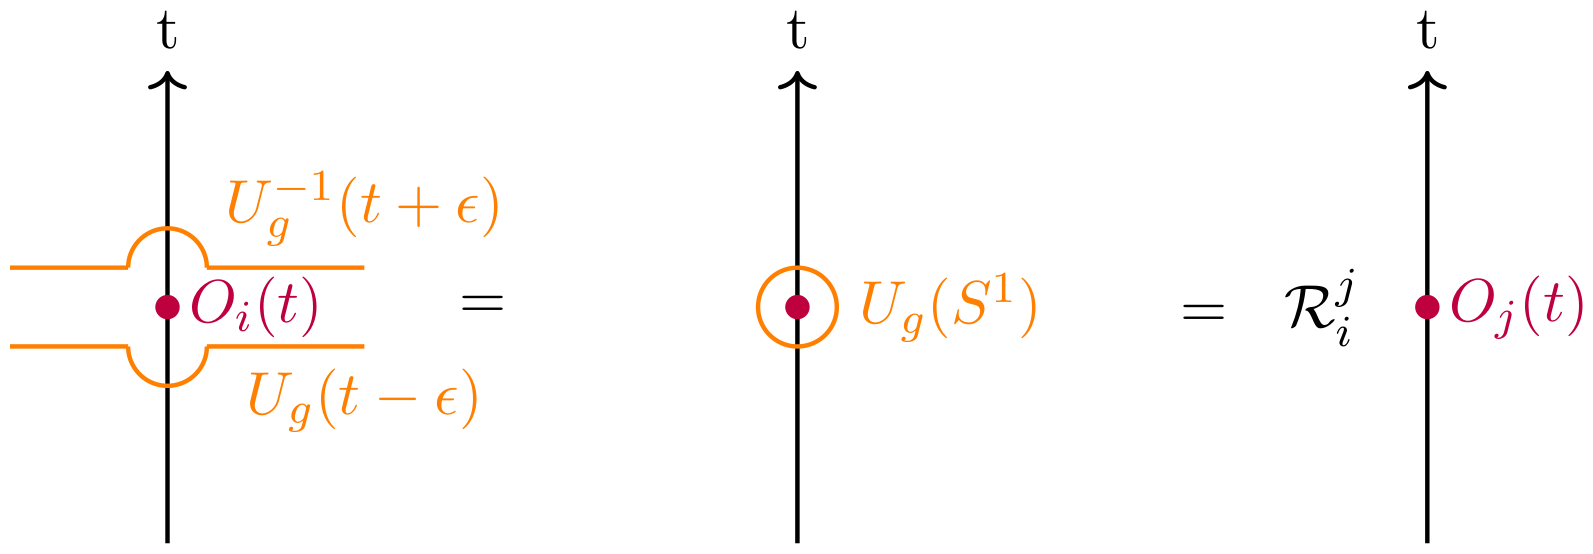
\includegraphics[width=0.62\linewidth]{figures/figure-2.png}
  % [原文图注为空]
  \caption{}
  \label{Fig:1FormQM}
\end{figure}

\begin{yizhu}上例到本例中“$U_g^{-1}$ 消失”只是画法的变化，并非定义改变：量子力学里 $U_g(t-\epsilon)$ 与 $U_g^{-1}(t+\epsilon)$ 是时间轴上夹住 $O_i(t)$ 的一对点插入，而 0-形式对称性把这对点“接”成一个闭合的 $S^{d-1}$（图~\ref{Fig:1FormQM} 左端即用一个环绕点算符的 $S^1$ 表示），闭合面上只剩一次插入，故作用律中不再显式出现逆算符。核对图~\ref{Fig:1FormQM} 时应看出：橙色圆环在时间轴上跨接并包住了原来上下两个插入点，于是 $\mathcal{R}(g)\mathcal{R}(g^{-1})=1$ 已在环内被用掉。\end{yizhu}

\begin{example}[$M^d$ 中的电磁学]
考虑 $d$ 维纯麦克斯韦理论中的 $U(1)$ 守恒流，
\[ \dd *F = j \]
于是
\[ U_g(M^{(d-1)}) = g^{\int_{M^{(d-1)}} j}  = \exp(i\alpha \int_{M^{(d-1)} } j ) \]
其中 $g = \exp(i\alpha)\in U(1)$ 是对称群的一个群元\footnote{事实上，前一情形中所说的 $U(1)$ 其实对应于 $U(1)$ 规范对称性的整体部分，即 $\alpha$ 与时空无关时的那一部分。}。
\end{example}

% ==== 原文 PDF 第 8 页 ====
若把 $M^{(d-1)}$ 取为一个时间切片，则 $\int_{M^{(d-1)} } j$ 就是该体系的总电荷。这一算符为何是拓扑的？这由 Stokes 定理给出。考虑对 $M^{(d-1)}$ 作一个小形变（小到没有点电荷穿过），记其为 $M^{(d-1)\prime}$，则
\[  \int_{M^{(d-1)}} j -  \int_{M^{(d-1)\prime}} j   = \int_{\partial D} j = \int_{D} \dd j = 0  \ , \]
其中 $D$ 是被形变部分所围的体积。$U_g$ 算符确实是拓扑的。

\begin{yizhu}记号预警：$\dd *F = j$ 中的 $j$ 是 $(d-1)$-形式，即电流 1-形式 $j_\mu$ 的 Hodge 对偶 $\star j$，而不是 $j_\mu$ 本身；因此 $\int_{M^{(d-1)}}j$ 是通量型积分。对照后文 (2.18) 写成 $\frac{1}{e^2}\dd *F = *j_E$ 就看得更清楚：那里右端显式带上星号，正是为了把 1-形式的电流 $j_E$ 与 $(d-1)$-形式的 $j$ 区分开。若把两处的 $j$ 混为一谈，会连带读错 (2.6) 与 (2.18) 中 $1/e^2$ 的归一化。\end{yizhu}

\subsection{高形式对称性}\label{sec:higher-form}

用拓扑算符的语言，向高形式对称性的推广是直截了当的：只需把与对称性算符相应的余维 $1$ 子流形（即 $d-1$ 维子流形）换成余维 $(p+1)$ 的流形，并把局域算符换成定义在 $p$ 维子流形上的对象（$p$ 维延展算符）。如此，拓扑算符记为 $U_g(M^{d-p-1})$，对象记为 $V(C^{p})$，则对称性对对象的作用为
\be
U_g(M^{d-p-1})V_i(C^p) = R_i {}^{j}(g) V_j(C^p) \ ,
\ee
前提是环绕数（linking number）$\langle M^{d-p-1},C^{p} \rangle = 1$。这里环绕数可直观地理解为两个子流形（维数之和为 $d-1$）在拓扑上相互缠绕而互不相交的方式；更清晰的定义是
\be
\langle M^{d-p-1},C^p \rangle = {\rm Int}(X^{d-p}, C^p) = {\rm Int}(M^{d-p-1}, Y^{p+1}) \ ,
\ee
其中 $\partial X^{d-p} = M^{d-p-1}$、$\partial Y^{p+1} = C^{p}$ 表明 $X^{d-p}$ 与 $Y^{p+1}$ 分别以 $M^{d-p-1}$ 与 $C^{p}$ 为边界，${\rm Int}$ 表示交点数（intersection number）。该公式的直观含义见下图。

\begin{center}
    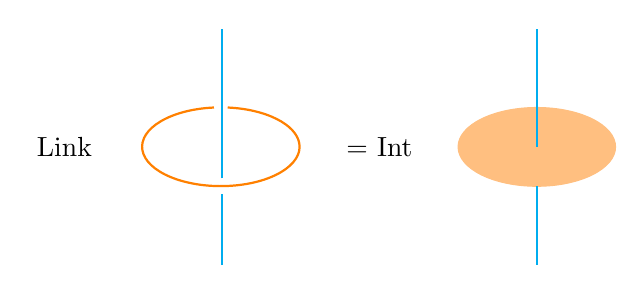
\begin{tikzpicture}
    \draw[thick, cyan] (-2,0.1)--(-2,2);
    \draw[thick, cyan] (-2,-1)--(-2,-0.1);
    \draw[thick, orange] (-2.1,1) arc (-265:85:1 and 0.5);
    \node[] at (0,0.5) {=  Int};
    \node[] at (-4,0.5) {Link};

    \filldraw[orange!50] (2.0,0.5) ellipse (1 and 0.5);
    \draw[thick, cyan] (2,0.5)--(2,2);
    \draw[thick, cyan] (2,0)--(2,-1);
    \end{tikzpicture}
\end{center}

\begin{yizhu}“相链”判据的两点提醒。其一，维数配平：$\dim M^{d-p-1}+\dim C^{p}=d-1$，故二者在 $d$ 维时空中一般不交；引入以 $M^{d-p-1}$ 为边界的 $X^{d-p}$ 后 $\dim X^{d-p}+\dim C^{p}=d$，横截相交为有限个点，故 $\langle M,C\rangle$ 等于交点数——这正是图中“Link $=$ Int”的含义。其二，交点数带定向符号：原文写 $\langle M^{d-p-1},C^{p}\rangle = 1$，使用时应理解为 $|\langle\cdot\rangle|=1$，相位 $\mathrm{e}^{in\alpha}$ 的符号取决于两子流形定向的选取。此外，原文 “The intuition for formula is” 一句在 PDF 中只接一幅图、未给文字说明，属原文行文疏略。\end{yizhu}

当然，作为作用在该体系上的对称群的表示，应当有
\be
U_g(M^{d-p-1})U_{g'}(M^{d-p-1})=U_{gg'}(M^{d-p-1}) \ .
\ee

\begin{yizhu}[原文疑误]此处有两处与源码/PDF 有关的细节。其一，源码把延展对象写作 $V_(C^{p})$（下划线直接接括号，TeX 会把它排成下标 $(C^{p})$），而 PDF 第 8 页实际排为 $V(C^{p})$；本译本从 PDF，恢复为 $V(C^{p})$。其二，本段原文作 “as a representation of the symmetric group”，按上下文（对称性算符的乘法律 $U_gU_{g'}=U_{gg'}$）应为 “symmetry group”；中文里两词都译作“对称群”，译文不显差别，但核对英文时勿误读为置换群 $S_n$。\end{yizhu}

接下来论证：若 $p>0$ 且时空拓扑平凡，则高形式对称性总是\textbf{阿贝尔的}。用拓扑算符的语言，这一论证几乎是显然的：
% ==== 原文 PDF 第 9 页 ====
设有两个余维 $\ge 2$ 的算符，就可以在时空中把二者作拓扑互换而没有任何障碍。图示情形见图~\ref{Fig:Abelian}。但在 $p=0$ 的情形无法作这样的互换，因为两个拓扑算符 $U_g$ 支撑在不同的时间切片上，它们一般可以不对易。

\begin{figure}[htbp]
  \centering
  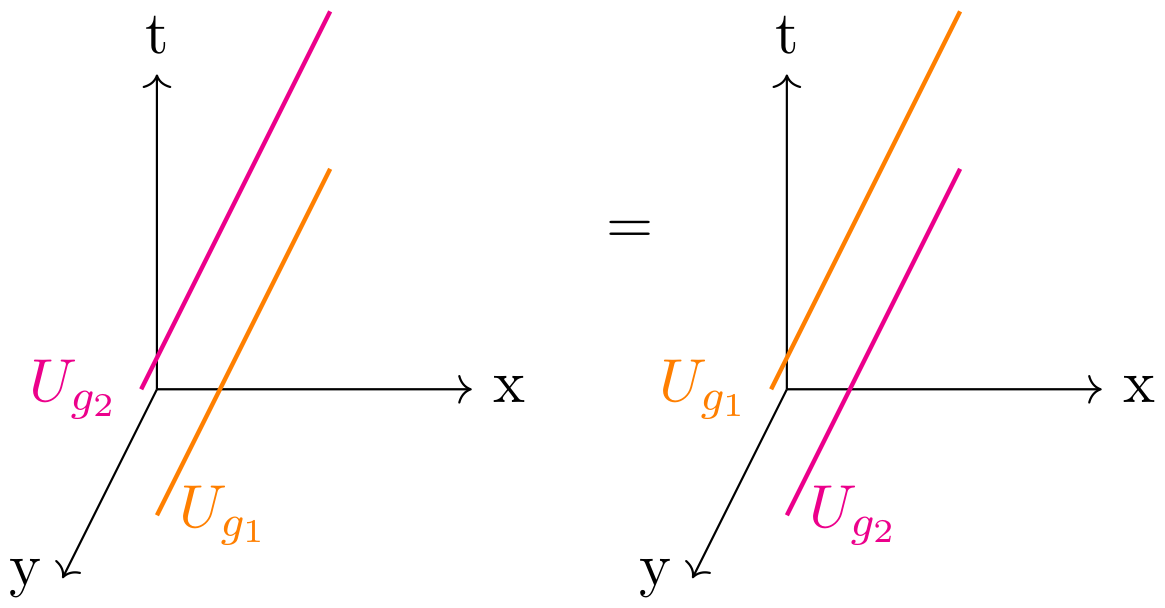
\includegraphics[width=0.46\linewidth]{figures/figure-3.png}
  \caption{在 $p>0$ 时交换拓扑算符。（原文 Figure~3，PDF 第 9 页）}
  \label{Fig:Abelian}
\end{figure}

\subsubsection{例：麦克斯韦理论}\label{subsec:Maxwell}

考虑 4 维纯 $U(1)$ 麦克斯韦理论，其作用量为
\be
S = \frac{1}{4e^2} \int {\rm d}^4 x \ F_{\mu\nu}F^{\mu\nu}
\ee
其中 $F_{\mu\nu} = \partial_\mu A_\nu- \partial_\nu A_\mu$，或等价地，$F = \frac{1}{2} F_{\mu\nu}{\rm d}x^\mu \wedge {\rm d}x^\nu = {\rm d}A $。众所周知，该理论具有 $U(1)_E \times U(1)_M$ 1-形式对称性。

下面说明 $U(1)_E$ 是 1-形式对称性：它由 $4-1-1=2$ 维拓扑算符生成，并作用在 1 维对象上。电的 $U(1)_E$ 对称性由拓扑算符
\be
\label{U1-UE}
U_E (S) = \exp(i\alpha Q_E(S))
\ee
生成，其中 $Q_E(S)$ 是 $S$ 所围的总电荷，即
\be
Q_E(S) = \frac{1}{e^2}\int_S *F = \frac{1}{e^2}\int_S \frac{\epsilon_{\mu\nu\rho\sigma}}{2!\cdot 2!}F^{\mu\nu} {\rm d}S^{\rho\sigma} \sim  \int_S \vb{E}\cdot \vb{{\rm d}S}\,.
\ee
该算符确实是拓扑的：由运动方程 ${\rm d}*F = 0 $，不碰到电荷的形变不会改变该算符。

那么算符所作用的对象是什么？答案是威尔逊圈（Wilson loop）。对给定的圈 $\gamma:[0,1]\to M, \gamma(1)=\gamma(0)$，威尔逊圈算符为
\be 
W_n(\gamma) = \exp(i n  \oint_\gamma A_\mu {\rm d}x^\mu )  = \exp(i n \int_\gamma A )\,. 
\ee
% ==== 原文 PDF 第 10 页 ====
拓扑算符 (\ref{U1-UE}) 对威尔逊圈的作用为（证明稍后在命题~\ref{Prop:1} 中给出）
\be
\expval{U_E(S) W_n(\gamma)} = \exp(in\alpha \expval{S,\gamma}) \expval{W_n(\gamma)}\,.
\ee

\textbf{注}：
\begin{enumerate}
\item 在威尔逊圈的定义中 $n\in \bbZ$。量子化的原因在于：在大规范变换 $A_\mu\mapsto A_\mu + \partial_\mu \epsilon$ 下，
    \[ \oint_\gamma \partial_\mu \epsilon {\rm d}x^\mu  = 2\pi k \quad \ k\in \bbZ\,, \]
    其中 $k$ 是绕数（winding number）。因此只有当 $n\in\mb{Z}$ 时，威尔逊圈才是规范不变的。
    
    \item 拓扑算符对威尔逊圈的这一作用，可等价地看作把 $A$ 平移一个平坦联络 $\lambda$（平坦指 ${\rm d}\lambda = 0$），即
    \be
    \oint_\gamma \lambda = \alpha \expval{S,\gamma}\,.
    \label{Eq:intlambda}\ee
    还应注意，该积分在 $\gamma$ 作小形变下不变。

    注意：即使 $\lambda$ 是平坦的，它也不能写成局域规范变换 $\lambda=d\epsilon$，否则对称性作用就是平凡的。
    
\end{enumerate}

现在转向与电对称性对偶的磁 $U(1)_M$ 对称性。这里的窍门很简单：给每样东西都配上 Hodge 星号 $*$。显然有
\be
U_M (S) = \exp(i\alpha Q_M(S))\,,
\ee
\be Q_M(S) = \frac{1}{2\pi}\int_S F = \frac{1}{4\pi}\int_S F_{\mu\nu} {\rm d}S^{\mu\nu} \sim  \int_S \vb{B}\cdot \vb{{\rm d}S} \,.
\ee
该算符是拓扑的，因为 ${\rm d}F = {\rm d^2}A = 0$。为构造威尔逊线的对偶版本，定义 $\tA$ 使得 ${\rm d}\tA = *\dd A $。于是 't Hooft 圈定义为
\be 
T_n(\gamma)  = \exp(i n \oint_\gamma \tA) = \exp(i n \oint_\gamma \tA_\mu \dd x^\mu)\,.
\ee
当然，$U_M$ 算符对 't Hooft 圈的作用为
\be
\expval{U_M(S) T_n(\gamma)} = \exp(in\alpha \expval{S,\gamma}) \expval{T_n(\gamma)}\,.
\ee
这也可以解释为把 $\tA$ 平移一个平坦联络。

\begin{prop}
\label{Prop:1}
\[ \expval{U_E(S) W_n(\gamma)} = \exp(in\alpha \expval{S,\gamma}) \expval{W_n(\gamma)}  \]
\end{prop}
% ==== 原文 PDF 第 11 页 ====
\begin{proof} 
\be {\rm L.H.S} = \int \mathscr{D}[A] \exp{iS + \frac{i\alpha}{e^2}\int_S *F + in \oint_\gamma A} \ee
这里的想法是对 $A$ 作一个平移：在此平移下测度 $\mathscr{D}[A]$ 不变，而指数上的各项只改变一个全导数项（在时空拓扑平凡的情形下无贡献），外加一个涉及环绕数的项。考虑
\begin{align*}
    \int_S *F &= \int_{V_S(\partial V_S = S)} d*F = \int_{V_S} \frac{\epsilon_{\nu\rho\sigma\tau}}{3!} \partial_\mu F^{\mu\nu} \dd v^{\rho\sigma\tau}\\
    &= \int \dd^4 x \ \partial_\mu F^{\mu\nu} J_\nu(V_S) = -\int\dd^4 x \ F^{\mu\nu} \partial_\mu J_\nu(V_S)
\end{align*} 
其中定义
\[ J_\nu(V_S) = \int_{V_S} \frac{\epsilon_{\nu\rho\sigma\tau}}{3!} \delta^4(x-y) \dd v^{\rho\sigma\tau}(y)\,. \]
可以看到这些项如何在 $A-\alpha J(V_S)$ 附近展开，相应结果为
\begin{align}
    W_n(\gamma,A) &= W_n(\gamma,A-\alpha J(V_S)) \exp(in\oint_\gamma J(V_S)) \\
    S[A] &= S[A-\alpha J(V_S)] + \frac{\alpha}{e^2} \int \dd^4 x \ \pmu J_\nu(V_S) \Fmn \ (+ {\rm higher\  derivative \ terms\ in\ }J_\mu) \ .
\end{align}

$J_\mu$ 中的高阶导数项不依赖于 $A$，因此作为归一化因子被略去。

最后，在作平移 $A\mapsto A-\alpha J(V_S)$ 之后，得到
\be
\expval{U_E(S) W_n(\gamma)} = \exp(in\alpha \oint_\gamma J(V_S)) \expval{W_n(\gamma)} \ .
\ee
由涉及交点数的定义可得
\[\oint_\gamma J(V_S) = \expval{S,\gamma}\,.\]

\end{proof}

\subsubsection{例：带荷物质的 $U(1)$ 规范理论}

现在给麦克斯韦理论加上带荷物质 $\{ \phi_i\}$，其电荷为 $q_i \in \bbZ$，即 $R_{q_i} (e^{i\alpha}) = e^{iq_i\alpha}$；同时定义正整数 $N = {\rm g.c.d}(q_i)$。

本情形的主要差别在于：$U(1)_E$ 的对称性流 $*F$ 不再守恒，取而代之的是
\be \frac{1}{e^2} \dd *F = *j_E \ , \ee
% ==== 原文 PDF 第 12 页 ====
其中 $j_E$ 是通常的电电流 1-形式。然而，若仍要求算符
\be U_E(e^{i\alpha}, S) = \exp(\frac{i\alpha}{e^2} \int_S *F) \ , \ee
是拓扑的，就要求 $S$ 的任意形变都保持不变，见图~\ref{fig:VS}。

\begin{figure}[htbp]
  \centering
  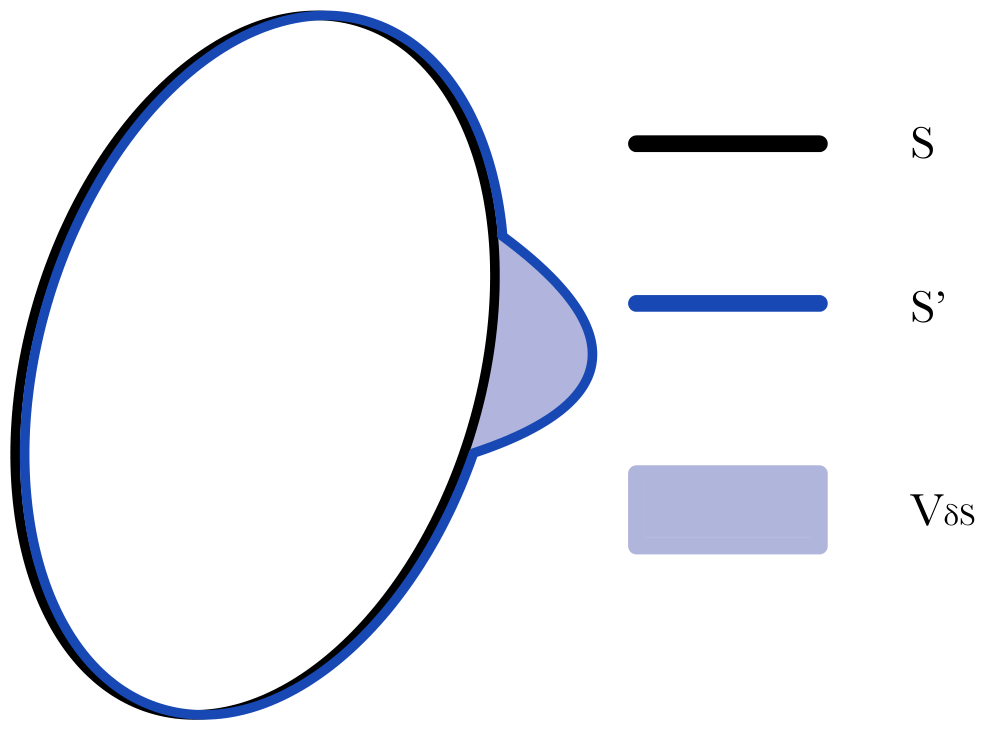
\includegraphics[width=0.39\linewidth]{figures/figure-4.png}
  \caption{本图展示从闭流形 $S$ 到 $S'$ 的形变：二者分别用黑色粗线与蓝色粗线标出。两个曲面会围出一个体积，该体积上的通量积分给出相应两个拓扑算符之差，见式~(2.20)。（原文 Figure~4，PDF 第 12 页）}
  \label{fig:VS}
\end{figure}

\be\ba 
U_E(e^{i\alpha}, S) &= U_E(e^{i\alpha}, S') \\
\Rightarrow \exp(\frac{i\alpha}{e^2}\int_{V_{\delta S}} \dd * F ) &= \exp(i\alpha\int_{V_{\delta S}} \ * j_E ) = 1 \quad \ptl V_{\delta S} = S \cup \overline{S'} \label{eq:VS}
\ea\ee

电荷量子化给出 $\int_{V_S} \ *j_E \in N\bbZ $，因此为满足 (\ref{eq:VS})，要求 $\alpha \in 2\pi \bbZ_N / N$。

\begin{yizhu}记号提醒：$\alpha \in 2\pi \bbZ_N / N$ 是原文的混写，字面上把群 $\mathbb{Z}_N$ 放到了整数集的位置。其实际含义是 $\alpha = 2\pi k/N$（$k\in\mathbb{Z}$，且 $\alpha$ 只定义到模 $2\pi$），即 $\alpha$ 取 $\mathbb{Z}_N$ 的 $N$ 个离散值；若读成“$\mathbb{Z}_N$ 的分数”便得不到对称性破缺到 $\mathbb{Z}_N$ 的结论。可与下文例~5 的结果对照：那里 $D=\mathrm{diag}(3,1)$，电对称性恰好破缺为 $\mathbb{Z}_3$。\end{yizhu}

因此，$U(1)_E$ 电 1-形式对称性群破缺为 $\bbZ_N$ 子群。还值得注意的是，在不包含磁单极子时，$U(1)_M$ 保持不变。

这一框架可以推广到带荷物质场 ${\phi_i}$ 的 $U(1)^r$ 规范理论。场 $\phi_i$ 在第 $j$ 个 $U(1)$ 对称性下的电荷为 $q_{i,j}\in\bbZ$。为计算对称性破缺，把荷矩阵记为 $Q = (q_{i,j})$，其中 $Q$ 不必是方阵。
% ==== 原文 PDF 第 13 页 ====
Smith 标准形分解（Smith normal decomposition）给出如下结果：
\be
\label{SmithDecomp}
U Q V = D = \begin{pmatrix}
d_1 &     &        &     &   &   &   \\
    & d_2 &        &     &   &   &   \\
    &     & \ddots &     &   &   &   \\
    &     &        & d_k &   &   &   \\
    &     &        &     & 0 & 0 & 0 & \cdots \\
    &     &        &     & 0 & 0 & 0 & \cdots
\end{pmatrix}\,.
\ee

这里 $U$ 与 $V$ 是元素为整数的可逆方阵。由此得到的 1-形式对称性为 $(\bigoplus_{i=1}^k \bbZ_{d_i})\oplus U(1)^{r-k} $。磁 1-形式对称性仍是 $U(1)_M=U(1)^r$。

\begin{yizhu}Smith 标准形 $UQV=D$ 的读法：$U,V$ 是整系数可逆方阵（$\det U=\pm1$、$\det V=\pm1$），左乘相当于重定义 $U(1)^r$ 规范荷的基底、右乘相当于重定义物质场基底，故不改变物理。对角元中只有 $d_i>1$ 的部分给出离散因子 $\mathbb{Z}_{d_i}$，$d_i=1$ 的因子不贡献；而 $Q$ 的秩之外的方向不被任何物质场带荷，剩下连续因子 $U(1)^{r-k}$。若 $Q$ 为满秩方阵，则 $\prod_i d_i=|\det Q|$，可用来快速验算：例如 (2.22) 的 $\det Q=3$ 正给出 $\mathbb{Z}_3$。\end{yizhu}

\begin{example}[具有 $\mb{Z}_3$ 电 1-形式对称性的理论]
作为例子，考虑 $U(1)^2$ 规范理论，其物质场的电荷为 $\phi_1=(2,-1)$、$\phi_2=(-1,2)$。
\end{example}

于是荷矩阵为
\be
Q=\bp 2 & -1\\-1 & 2\ep\,.
\ee
经过 Smith 标准形分解得到 $D=\rm{diag}(3,1)$，因此电 1-形式对称性破缺为 $\mb{Z}_3$ 子群。

事实上，这恰好是纯 $SU(3)$ 规范理论的库仑相（Coulomb phase）。

\subsubsection{4 维非阿贝尔规范理论}

另一类众所周知的例子是非阿贝尔规范理论，读者可参阅 David Tong 的规范理论讲义~\cite{TongGauge}。为简单起见，考虑规范群为 $G$ 的纯杨–米尔斯理论。

对 $G = SU(N)$，$\bbZ_N$ 是由 $SU(N)$ 的中心生成的 1-形式电对称性，它作用在对此对称性带荷的威尔逊圈上。

下面讨论 $S^1\times\mb{R}^3$ 上的有限温度体系，其中欧氏时间圆满足 $x^0\sim x^0+\beta$。$\mb{Z}_N$ 1-形式中心对称性由函数的等价类 $[h_k]=\{h_k(x^\mu)\in SU(N), h_k(x^\mu)\sim g(x^\mu)h_k(x^\mu)g^{-1}(x^\mu)\}$ 定义，该等价类到 $SU(N)$ 的中心为止是周期的：$h_k(x^0=\beta)=e^{2\pi k/N}h_k(x^0=0)$。它对 $A$ 的作用为
\be
A\rightarrow h_kAh_k^{-1}+h_kdh_k^{-1}\,,
\ee
该作用在局域算符上是平凡的，但在 Polyakov 圈
\be
P_R=\text{tr}_R(\mathcal{P}\exp\left(\oint_{S^1}A^0\right)
\ee
上非平凡：
\be
P_R\rightarrow P_R e^{\frac{2\pi i k n_R}{N}}\,.
\ee
% ==== 原文 PDF 第 14 页 ====
其中 $R$ 是 $SU(N)$ 的表示，它定义了威尔逊圈（Polyakov 圈）；$n_R$ 称为“$N$-性”（N-ality），等于 $R$ 的杨图中方框总数模 $N$。

$\mb{Z}_N$ 1-形式对称性的这一作用也适用于一般的威尔逊圈：
\be
\ba
U_{k(\in \bbZ_N)}(S^2) W_R(\gamma) &= W_R(\gamma) \Big[A + \frac{2\pi k}{N} I \Big] \quad \expval{S^2 ,\gamma} = 1\cr
&=e^{\frac{2\pi ik n_R}{N}}W_R(\gamma)\,.
\ea
\ee

在 $G = PSU(N) = SU(N)/\bbZ_N$ 的情形，体系表现出作用在 't Hooft 圈上的 $\bbZ_N$ 磁对称性，原因在于 $\pi_1(PSU(N))=\mb{Z}_N$~\cite{TongGauge}。下面的描述可以说明这一点。考虑纯空间中的磁单极子（在时空中即 't Hooft 线）；吴–杨磁单极子构造告诉我们，把空间分为北/南半球后，规范势为
\be\ba
A_N = &B_0 \frac{1+\cos(\theta)}{2 r^2} \dd \phi \\
A_S = &B_0 \frac{-1+\cos(\theta)}{2 r^2} \dd \phi \\
\ea\ee
而赤道处的拼接条件为
\be \exp(i B_0\phi) =  \exp(i B_0(\phi+2\pi) )\Rightarrow \exp(2\pi i B_0 ) = I_{PSU(N)} \ee
这样的 $B_0$ 选择由 $\pi_1(PSU(N)) = \bbZ_N$ 分类。

我们指出：在 $SU(N)$ 理论中存在中心 $\bbZ_N^{(1)}$ 对称性，但没有这种磁对称性，因为 $\pi_1(SU(N)) = 0$。而在 $PSU(N)$ 理论中没有中心对称性（其中心平凡），但有磁 $\bbZ_N^{(1)}$ 对称性。这一关系可以推广，见~\cite{Brennan:2023mmt}。

更一般地说，在规范李代数为 $\mathfrak{su}(N)$ 的纯杨–米尔斯理论中，可以用荷 $(n_E,n_M)\in \bbZ_N\times \bbZ_N$ 对圈算符分类。荷为 $(n_E,n_M)$ 与 $(n_E',n_M')$ 的两个这类算符相互局域（从而可以共存），当且仅当它们满足狄拉克量子化条件
\be
n_E n_M'-n_M n_E'=0\quad (\text{mod}\ N)\,.
\ee
这样一组互局域算符的选取称为\textbf{极化}（polarization）。例如，若选取全部威尔逊圈作为互局域算符集合，则该规范理论的整体形式是 $G=SU(N)$ 规范理论；相反，若选取全部 't Hooft 圈，则整体形式是 $G=PSU(N)$ 规范理论。当然，当 $N$ 不是素数时，还可以有介于两者之间的情形。

% ==== 原文 PDF 第 15 页 ====
选定极化之后，该理论称为\textbf{绝对理论}（absolute theory），其配分函数良定义；否则一般称为\textbf{相对理论}（relative theory），只有配分向量。配分向量的概念最早是在 6 维 (2,0) 理论及其环面紧致化的语境中引入的，那里存在互不局域的双子（dyonic）带荷算符，详见~\cite{Witten:2009at,Freed:2012bs,Tachikawa:2013hya}。
